%appendix
\chapter{Supplementary Material}

\section{Theory}

\begin{figure}
  \begin{tikzpicture}[
declare function={gamma(\z)=
2.506628274631*sqrt(1/\z)+ 0.20888568*(1/\z)^(1.5)+ 0.00870357*(1/\z)^(2.5)- (174.2106599*(1/\z)^(3.5))/25920- (715.6423511*(1/\z)^(4.5))/1244160)*exp((-ln(1/\z)-1)*\z;},
declare function={gammapdf(\x,\k,\theta) = 1/(\theta^\k)*1/(gamma(\k))*\x^(\k-1)*exp(-\x/\theta);}]
\begin{axis}[ymode=log, ymin=0,
no markers, domain=0:9, samples=100,
axis lines=left, xlabel=$\text{TS}$, ylabel=$\#\text{trials}$,
y label style={at={(axis description cs:-0.1,.5)},anchor=north},
x label style={dashed,at={(axis description cs:0.95,-0.1)},anchor=west},
height=5cm, width=9cm,
xtick={6,14.87}, ytick=\empty,
xticklabels={$\text{bg median}$,$5\sigma$},
%xticklabels={$\bar n (\theta_t)$},
enlargelimits=false, clip=false,% axis on top,
grid = major]
\addplot [very thick,cyan!20!black,domain=0:20, draw=none] {gammapdf(x,0.2,5)};
\addplot [very thick,cyan!20!black,domain=0.5:19.5] {gammapdf(x,0.2,5)};
%\addplot [domain= 0.5:4.5]{gauss(2.5,0.6,2)};
%\addplot [fill=cyan!20, draw=none, domain=0:6.0] {gammapdf(x,2,2)} \closedcycle;
%\addplot [very thick, fill=white!20!white, draw=none, domain=6.01:20] {gammapdf(x,2,2)} \closedcycle;
\end{axis}
\node at (2.5,1.7) {\begin{tikzpicture} \begin{axis}[hide axis,enlargelimits=false, ymax = 1,height=5cm, width=4cm,domain=2.65:3.35]\addplot [domain= 2.65:3.35,smooth,thick,green]{gauss(3,0.1,0.2)}; \end{axis} \end{tikzpicture}};
\node at (5.5,1.7) {\begin{tikzpicture} \begin{axis}[hide axis,enlargelimits=false, ymax = 1,height=5cm, width=3.5cm,domain=2.7:3.3]\addplot [domain= 2.7:3.3,smooth,thick,red]{gauss(3,0.07,0.14)}; \end{axis} \end{tikzpicture}};
\node[green] at (2.7,3) {$\xrightarrow{\text{90\%}}$};
\node[red] at (6,3) {$\xrightarrow{\text{50\%}}$};
\node at (0.5,3) {$\text{bg}$};
\node[green] at (2.7,4) {$\text{sensitivity}$};
\node[red] at (6,4) {$\text{discovery}$};
\end{tikzpicture}
\caption{Schematic showing the conditions to calculate the sensitivity and discovery potential. The background test statistic is shown in black, the signal test statistic satisfying the sensitivity conditions in green and the one for the discovery potential in red. Note that the curves dont actually look like these shown here. They have been simplified for explanatory purpose.}
\label{fig:sens_disc_schem}
\end{figure}

\section{Sources}

\begin{figure}
    \centering
    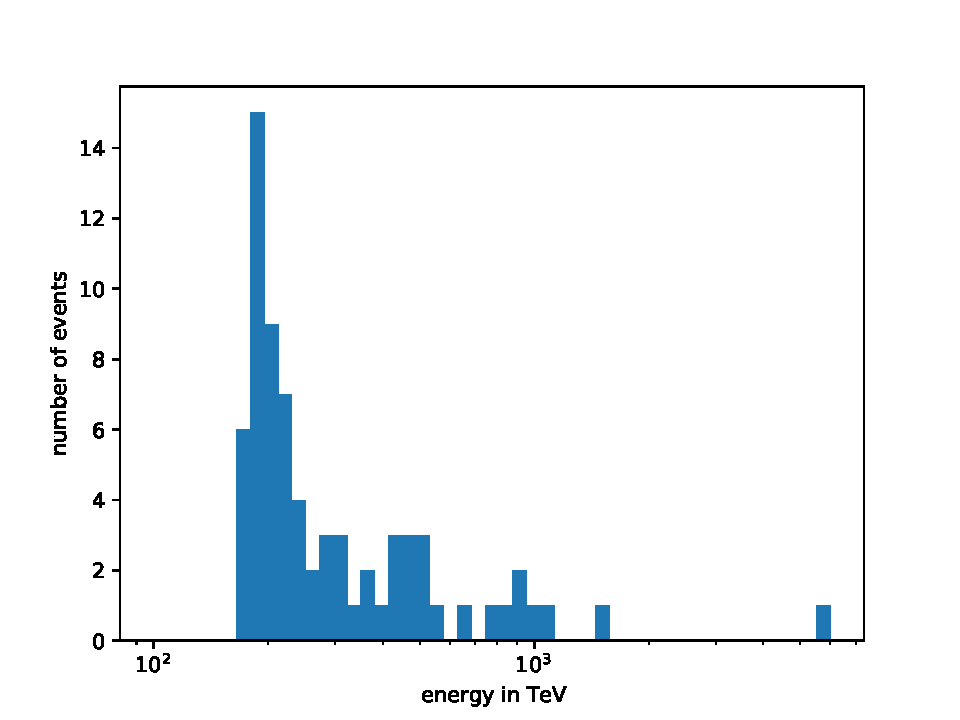
\includegraphics[width=\linewidth]{Plots/appendix/sources_energy.pdf}
    \caption{Histogram of the energy of the used sources seen in table \ref{tab:sources} in $\si{\tera\electronvolt}$.}
    \label{fig:sources_energy}
\end{figure}

\begin{table}
  \centering
  \caption{Table of the sources used in the time-dependent analysis. Additionally the signalness parameter is shown after which the sources were selected.}
  \label{tab:sources_time_dep}
  \begin{tabular}{ccrrc}
    \toprule
    Nr. & MJD &  $\delta$ in $\si{\degree}$ & $\alpha$ in $\si{\degree}$ & signalness in $\si{\percent}$ \\
    \toprule
      11 & 56819.20 & 11.45 & 110.65 & 99.70 \\ 12 & 56470.11 & 14.17 & 93.74 & 93.80 \\ 13 & 57951.82 & 25.16 & 208.39 & 86.60 \\ 16 & 58063.78 & 7.44 & 340.14 & 97.50 \\ 29 & 57340.87 & 12.71 & 76.16 & 95.70 \\ 37 & 55911.28 & 18.88 & 36.74 & 94.60 \\ 42 & 56226.60 & 27.91 & 169.80 & 92.60 \\ 43 & 56666.50 & 33.02 & 293.12 & 92.70 \\ 58 & 57478.57 & 15.48 & 151.22 & 85.10 \\ 63 & 56211.77 & -2.28 & 205.14 & 84.20 \\ 
    \toprule
  \end{tabular}
\end{table}

\section{Time-Integrated Search}

\begin{table}
  \centering
  \caption{Table of the number of injected signal events used for the time integrated analysis.}
  \label{tab:sig_time_int_table}
  \begin{tabular}{r}
    \toprule
    $n_\text{S}$ injected \\
    \toprule
      0.0 \\ 7.5 \\ 15.0 \\ 22.5 \\ 30.0 \\ 36.0 \\ 57.0 \\ 78.0 \\ 99.0 \\ 120.0 \\ 141.0 \\ 194.2 \\ 247.4 \\ 300.7 \\ 353.9 \\ 407.1 \\ 460.3 \\ 513.6 \\ 566.8 \\ 620.0 \\ 
    \toprule
  \end{tabular}
\end{table}

\begin{table}
  \caption{Table of the number of trials for each spectral index $\gamma$ and number of injected signal events $n_\text{sig}$, running $\num{10}$ jobs with $\num{5e3}$ trials per set of parameter pairs $\gamma$ and $n_\text{sig}$. Some jobs fail due to technical reasons.}
  \label{tab:trials_sig_time_int_table}
  \begin{subtable}{\linewidth}
  \centering
  \begin{tabular}{p{.9cm}|rrrrrrrrrr}
    \toprule
    \: $n_\text{sig}$ \newline $\gamma$ \: & 0.0 & 7.5 & 15.0 & 22.5 & 30.0 & 36.0 & 57.0 & 78.0 & 99.0 & 141.0 \\ 
    \toprule
    1.50 & 50000 & 50000 & 50000 & 50000 & 50000 & 50000 & 50000 & 50000 & 50000 & 50000 \\ 1.75 & 50000 & 50000 & 50000 & 50000 & 50000 & 50000 & 50000 & 50000 & 50000 & 50000 \\ 2.00 & 50000 & 50000 & 50000 & 50000 & 50000 & 50000 & 50000 & 50000 & 50000 & 50000 \\ 2.25 & 50000 & 45000 & 45000 & 45000 & 50000 & 45000 & 50000 & 50000 & 50000 & 50000 \\ 2.50 & 50000 & 50000 & 50000 & 50000 & 50000 & 50000 & 50000 & 50000 & 50000 & 50000 \\ 2.75 & 50000 & 50000 & 45000 & 45000 & 50000 & 50000 & 50000 & 40000 & 50000 & 40000 \\ 3.00 & 50000 & 50000 & 50000 & 50000 & 50000 & 45000 & 50000 & 50000 & 50000 & 50000 \\ 
    \toprule
  \end{tabular}
\end{subtable}
\begin{subtable}{\linewidth}
\centering
  \begin{tabular}{p{.9cm}|rrrrrrrrrr}
    \toprule
    \: $n_\text{sig}$ \newline $\gamma$ \: & 141.0 & 194.2 & 247.4 & 300.7 & 353.9 & 407.1 & 460.3 & 513.6 & 566.8 & 620.0 \\ 
    \toprule
    1.50 & 50000 & 50000 & 50000 & 50000 & 50000 & 50000 & 50000 & 50000 & 50000 & 50000 \\ 1.75 & 50000 & 50000 & 50000 & 50000 & 50000 & 50000 & 50000 & 50000 & 50000 & 45000 \\ 2.00 & 50000 & 50000 & 50000 & 50000 & 50000 & 50000 & 50000 & 50000 & 50000 & 50000 \\ 2.25 & 50000 & 50000 & 50000 & 50000 & 50000 & 50000 & 50000 & 50000 & 50000 & 50000 \\ 2.50 & 50000 & 50000 & 50000 & 50000 & 50000 & 50000 & 50000 & 50000 & 50000 & 40000 \\ 2.75 & 50000 & 50000 & 50000 & 50000 & 50000 & 50000 & 50000 & 50000 & 50000 & 50000 \\ 3.00 & 50000 & 50000 & 45000 & 50000 & 50000 & 50000 & 50000 & 50000 & 50000 & 50000 \\ 
    \toprule
  \end{tabular}
  \end{subtable}
\end{table}

\section{Time-Dependent Search}

\begin{table}
  \centering
  \caption{Table of the number of trials for each spectral index source index number and number of injected signal events $n_\text{sig}$, running $\num{5}$ jobs with $\num{e4}$ trials per set of parameter pairs of source and $n_\text{sig}$. Some jobs fail due to technical reasons.}
  \label{tab:trials_sig_time_dep_table}
  \begin{tabular}{>{\centering\arraybackslash}p{.9cm}|%
                    cccccccccc}
    \toprule
    \: Nr. \newline $n_\text{sig}$ \: & 11 & 12 & 13 & 16 & 29 & 37 & 42 & 43 & 58 & 63 \\ 
    \toprule
    0.0 & 50000 & 50000 & 50000 & 50000 & 50000 & 10000 & 40000 & 50000 & 50000 & 30000 \\ 1.1 & 50000 & 50000 & 50000 & 50000 & 50000 & 20000 & 40000 & 50000 & 50000 & 20000 \\ 2.2 & 50000 & 50000 & 50000 & 50000 & 50000 & 0 & 40000 & 50000 & 50000 & 30000 \\ 3.3 & 50000 & 50000 & 40000 & 50000 & 50000 & 50000 & 40000 & 50000 & 50000 & 30000 \\ 4.4 & 50000 & 50000 & 30000 & 50000 & 50000 & 40000 & 50000 & 50000 & 50000 & 10000 \\ 5.6 & 50000 & 40000 & 30000 & 50000 & 50000 & 40000 & 50000 & 50000 & 50000 & 20000 \\ 6.7 & 50000 & 40000 & 30000 & 50000 & 50000 & 50000 & 50000 & 50000 & 50000 & 50000 \\ 7.8 & 50000 & 50000 & 30000 & 50000 & 50000 & 50000 & 50000 & 50000 & 50000 & 50000 \\ 8.9 & 50000 & 50000 & 30000 & 20000 & 40000 & 50000 & 50000 & 50000 & 50000 & 40000 \\ 10.0 & 50000 & 50000 & 30000 & 40000 & 50000 & 50000 & 50000 & 50000 & 50000 & 50000 \\ 12.0 & 50000 & 50000 & 50000 & 30000 & 50000 & 50000 & 50000 & 50000 & 50000 & 50000 \\ 14.0 & 50000 & 50000 & 50000 & 20000 & 50000 & 50000 & 50000 & 50000 & 50000 & 50000 \\ 16.0 & 50000 & 40000 & 50000 & 30000 & 50000 & 50000 & 50000 & 50000 & 50000 & 50000 \\ 18.0 & 50000 & 50000 & 50000 & 40000 & 50000 & 50000 & 50000 & 50000 & 50000 & 50000 \\ 20.0 & 50000 & 50000 & 50000 & 40000 & 50000 & 40000 & 50000 & 50000 & 50000 & 40000 \\ 22.0 & 50000 & 50000 & 50000 & 50000 & 50000 & 30000 & 50000 & 50000 & 50000 & 50000 \\ 24.0 & 50000 & 50000 & 50000 & 50000 & 50000 & 30000 & 50000 & 50000 & 50000 & 50000 \\ 26.0 & 50000 & 50000 & 50000 & 50000 & 50000 & 30000 & 50000 & 50000 & 50000 & 50000 \\ 28.0 & 50000 & 50000 & 50000 & 50000 & 50000 & 40000 & 50000 & 50000 & 50000 & 50000 \\ 30.0 & 50000 & 50000 & 50000 & 50000 & 30000 & 20000 & 50000 & 50000 & 50000 & 50000 \\ 
    \toprule
  \end{tabular}
\end{table}

\begin{figure}
    \centering
    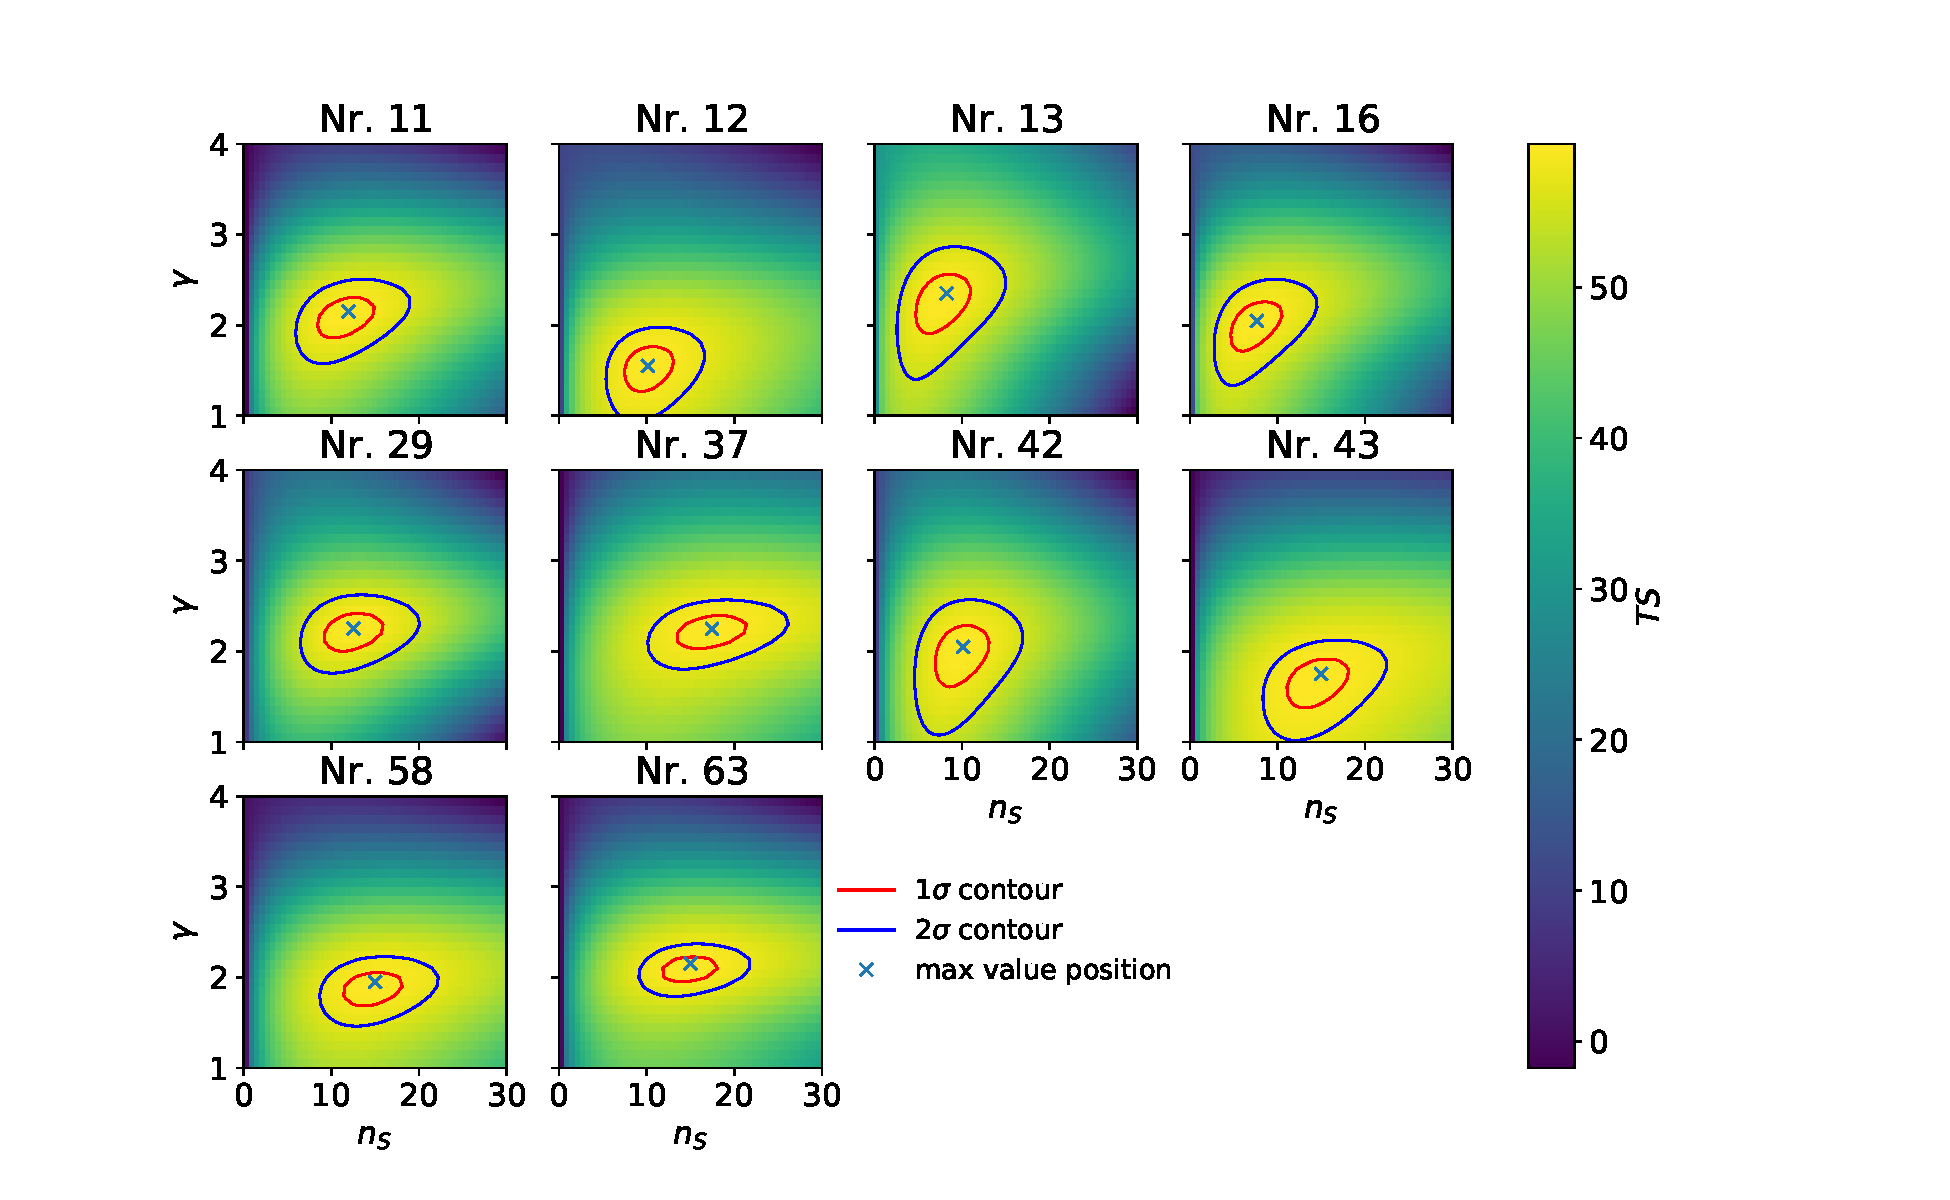
\includegraphics[width=\linewidth]{Plots/appendix/llh_scan.pdf}
    \caption{Scan of the likelihoodspace for all $\num{10}$ sources with a timewindow of $\SI{200}{\day}$ for the time-dependent analysis. The scan is in the spectral index $\gamma$ and the signal parameter $n_\text{S}$. The number of induced signal events is $n_S = \num{10}$ with a spectral index of $\gamma = 2$. The maximum test statistic value is marked in the plot including the contours of $\num{1}\sigma$ and $\num{2}\sigma$ and source number corresponds to table \ref{tab:sources}.}
    \label{fig:llh_scan_time_dep_all}
\end{figure}

\begin{figure}
    \centering
    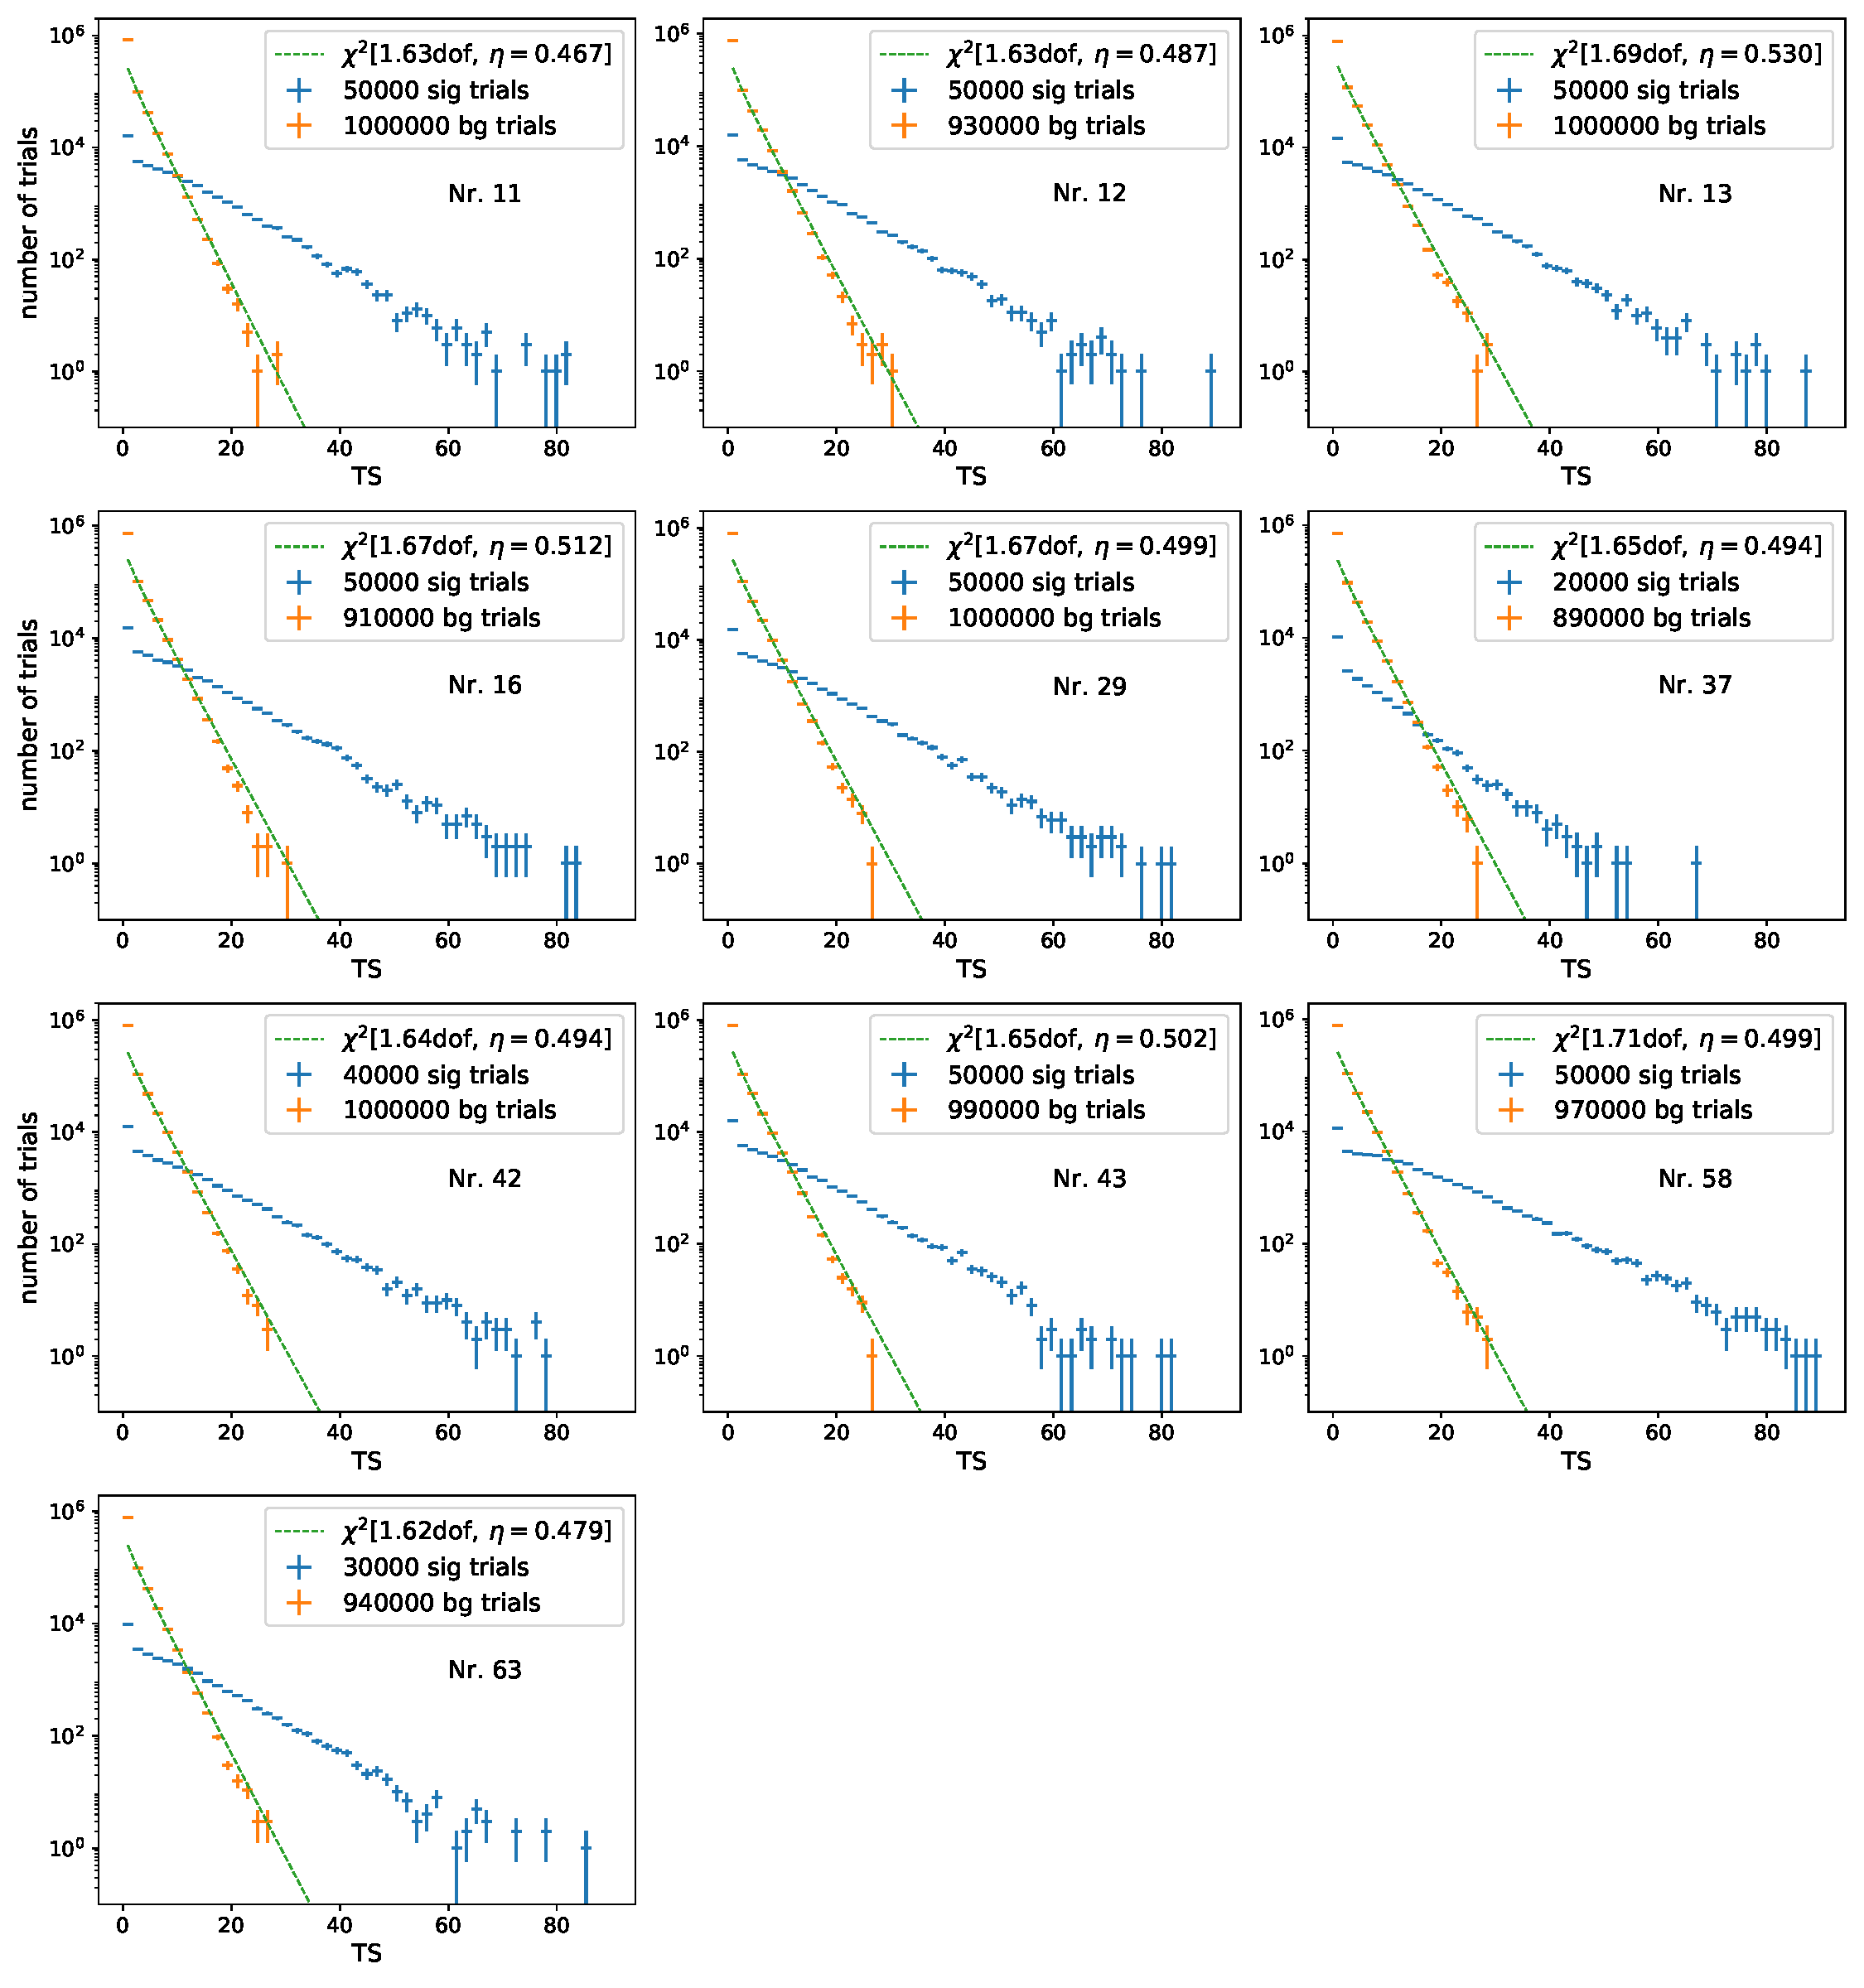
\includegraphics[width=\linewidth]{Plots/appendix/9_years_gfu_gold_time_dep_sig_sens_ts.pdf}
    \caption{Histogram of the background trials for the time-dependent analysis for all $\num{10}$ sources. Shown is also the set of signal trials with the number of injected signal events closest to satisfying the condition to calculate the sensitivity. The median of the background test statistics is not plotted as it is very close to the origin for all sources.}
    \label{fig:time_dep_sig_sens_ts}
\end{figure}

\begin{figure}
    \centering
    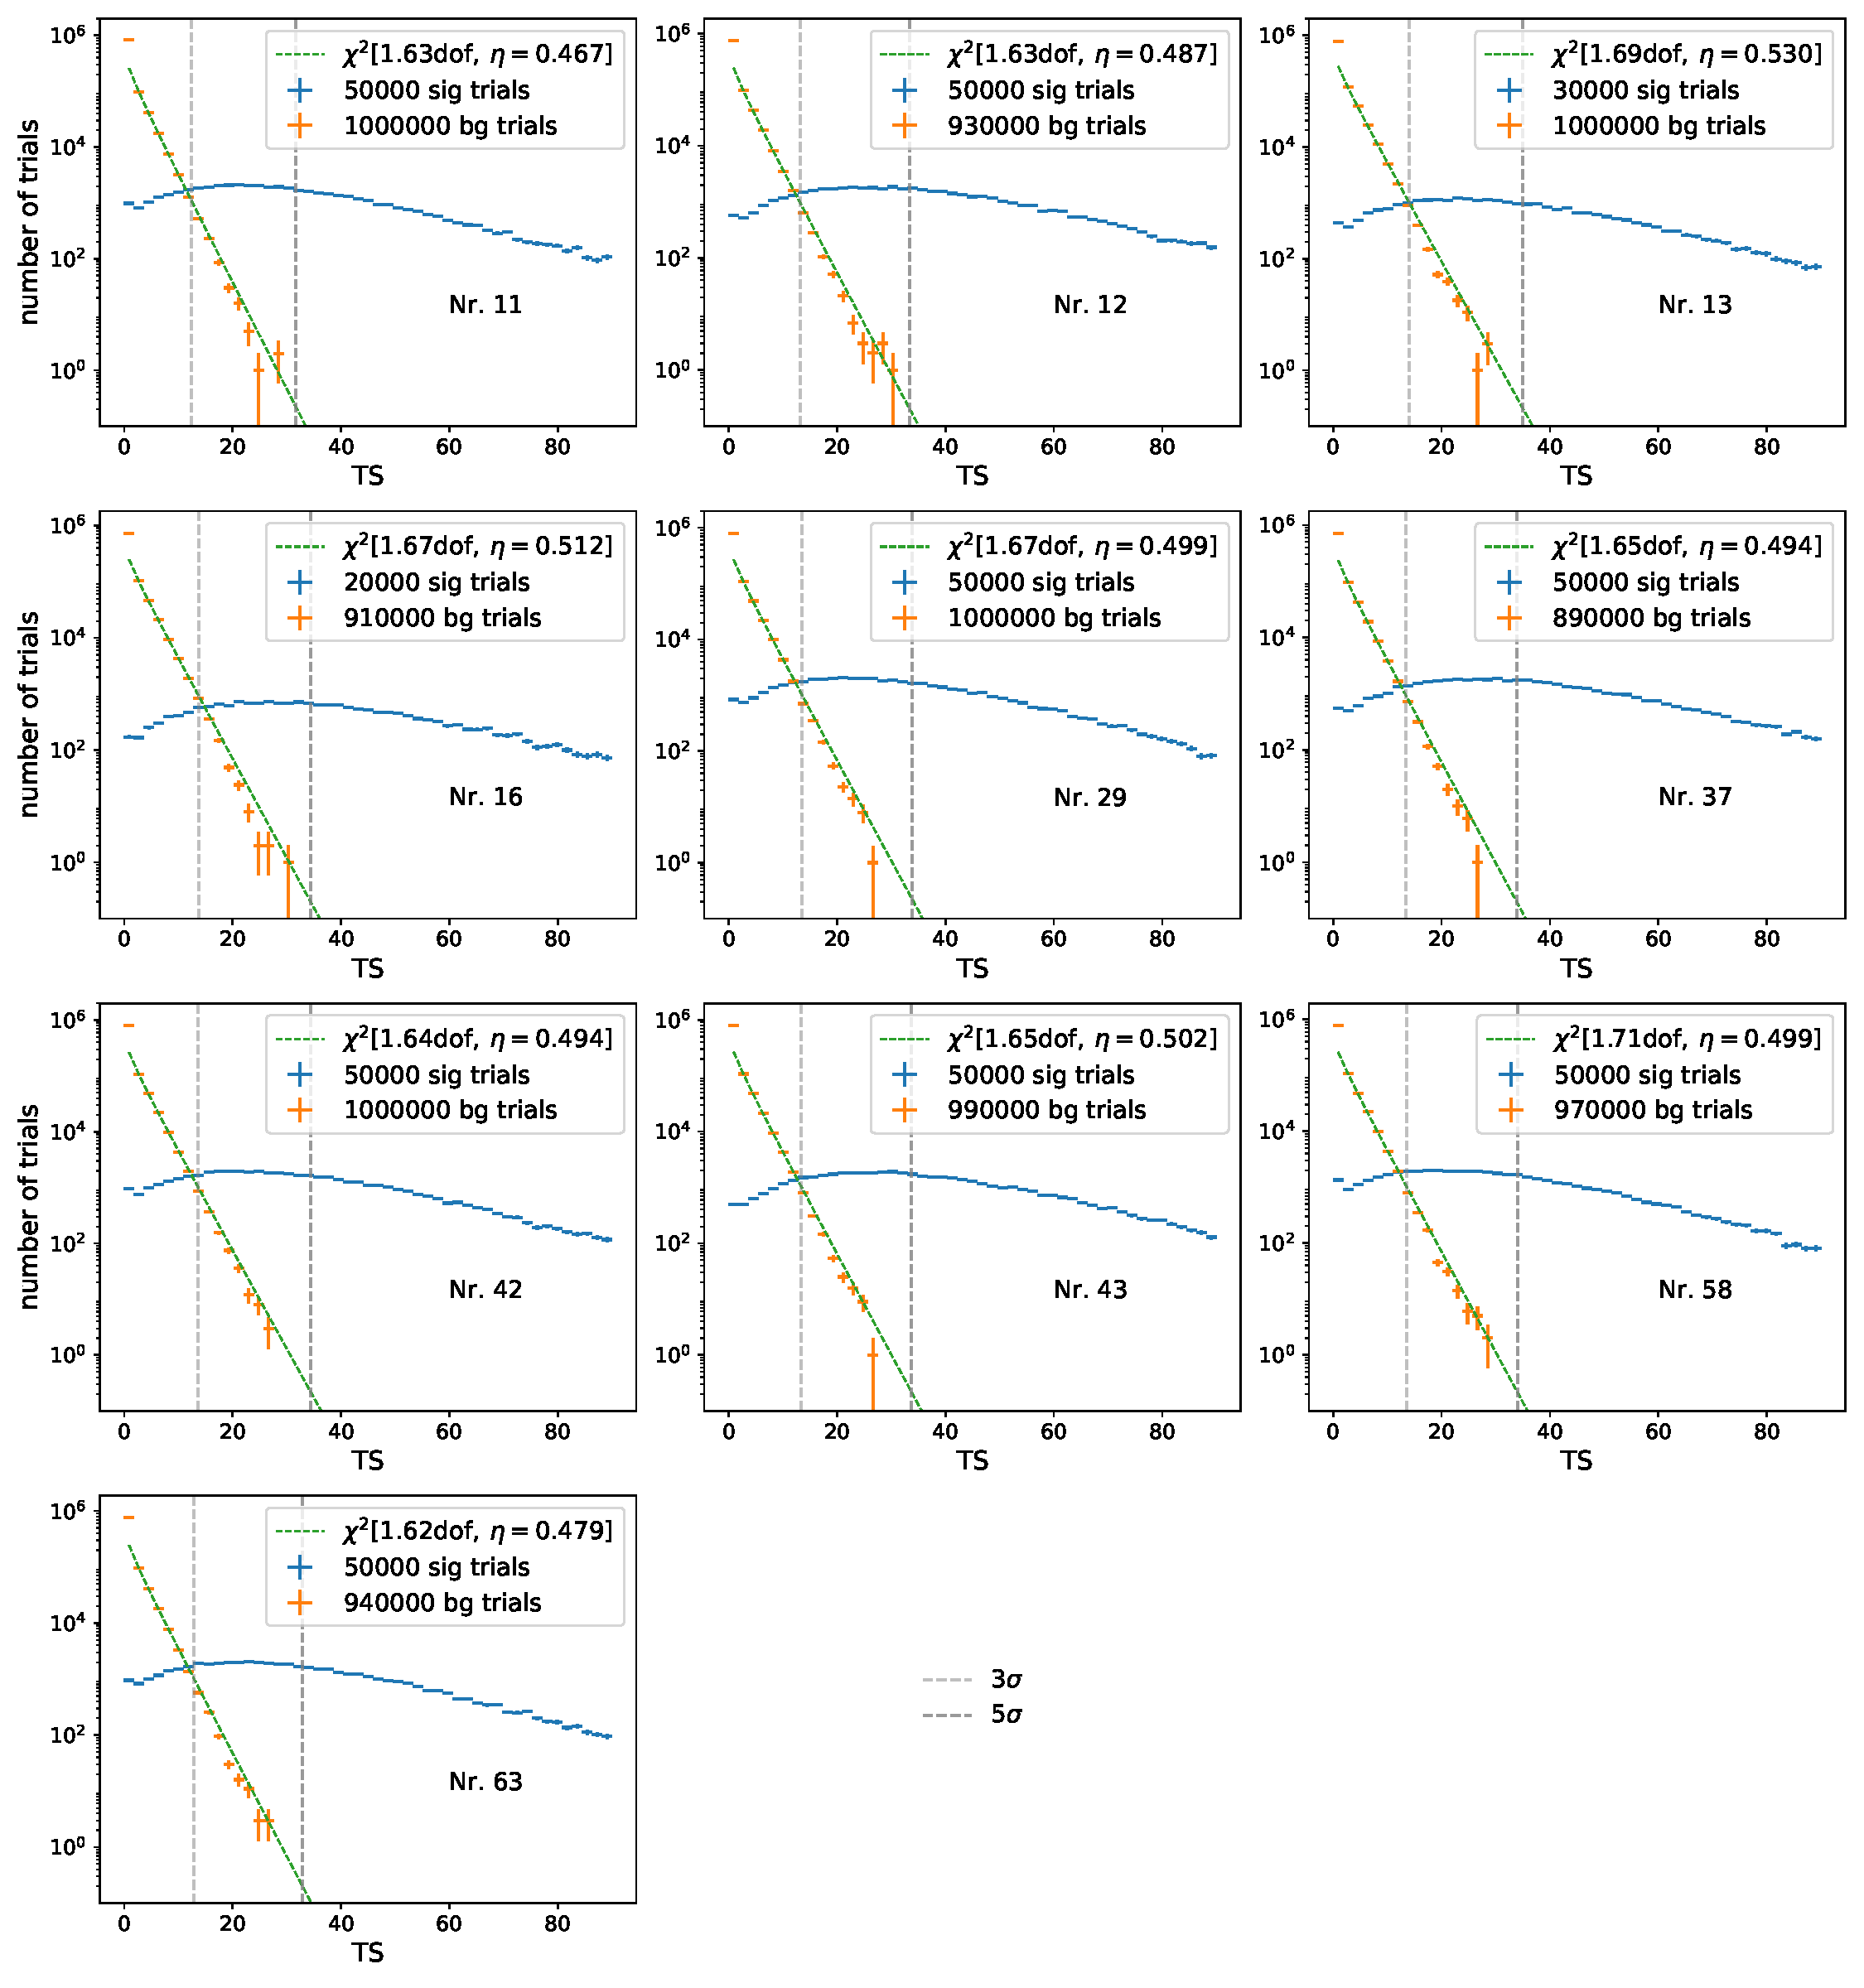
\includegraphics[width=\linewidth]{Plots/appendix/9_years_gfu_gold_time_dep_sig_disc_ts.pdf}
    \caption{Histogram of the background trials for the time-dependent analysis for all $\num{10}$ sources. Shown is also the set of signal trials with the number of injected signal events closest to satisfying the condition to calculate the discovery potential. The grey dashed lines represent $\num{3}\sigma$ and $\num{5}\sigma$ of the background teststatistic.}
    \label{fig:time_dep_sig_disc_ts}
\end{figure}

\begin{figure}
    \centering
    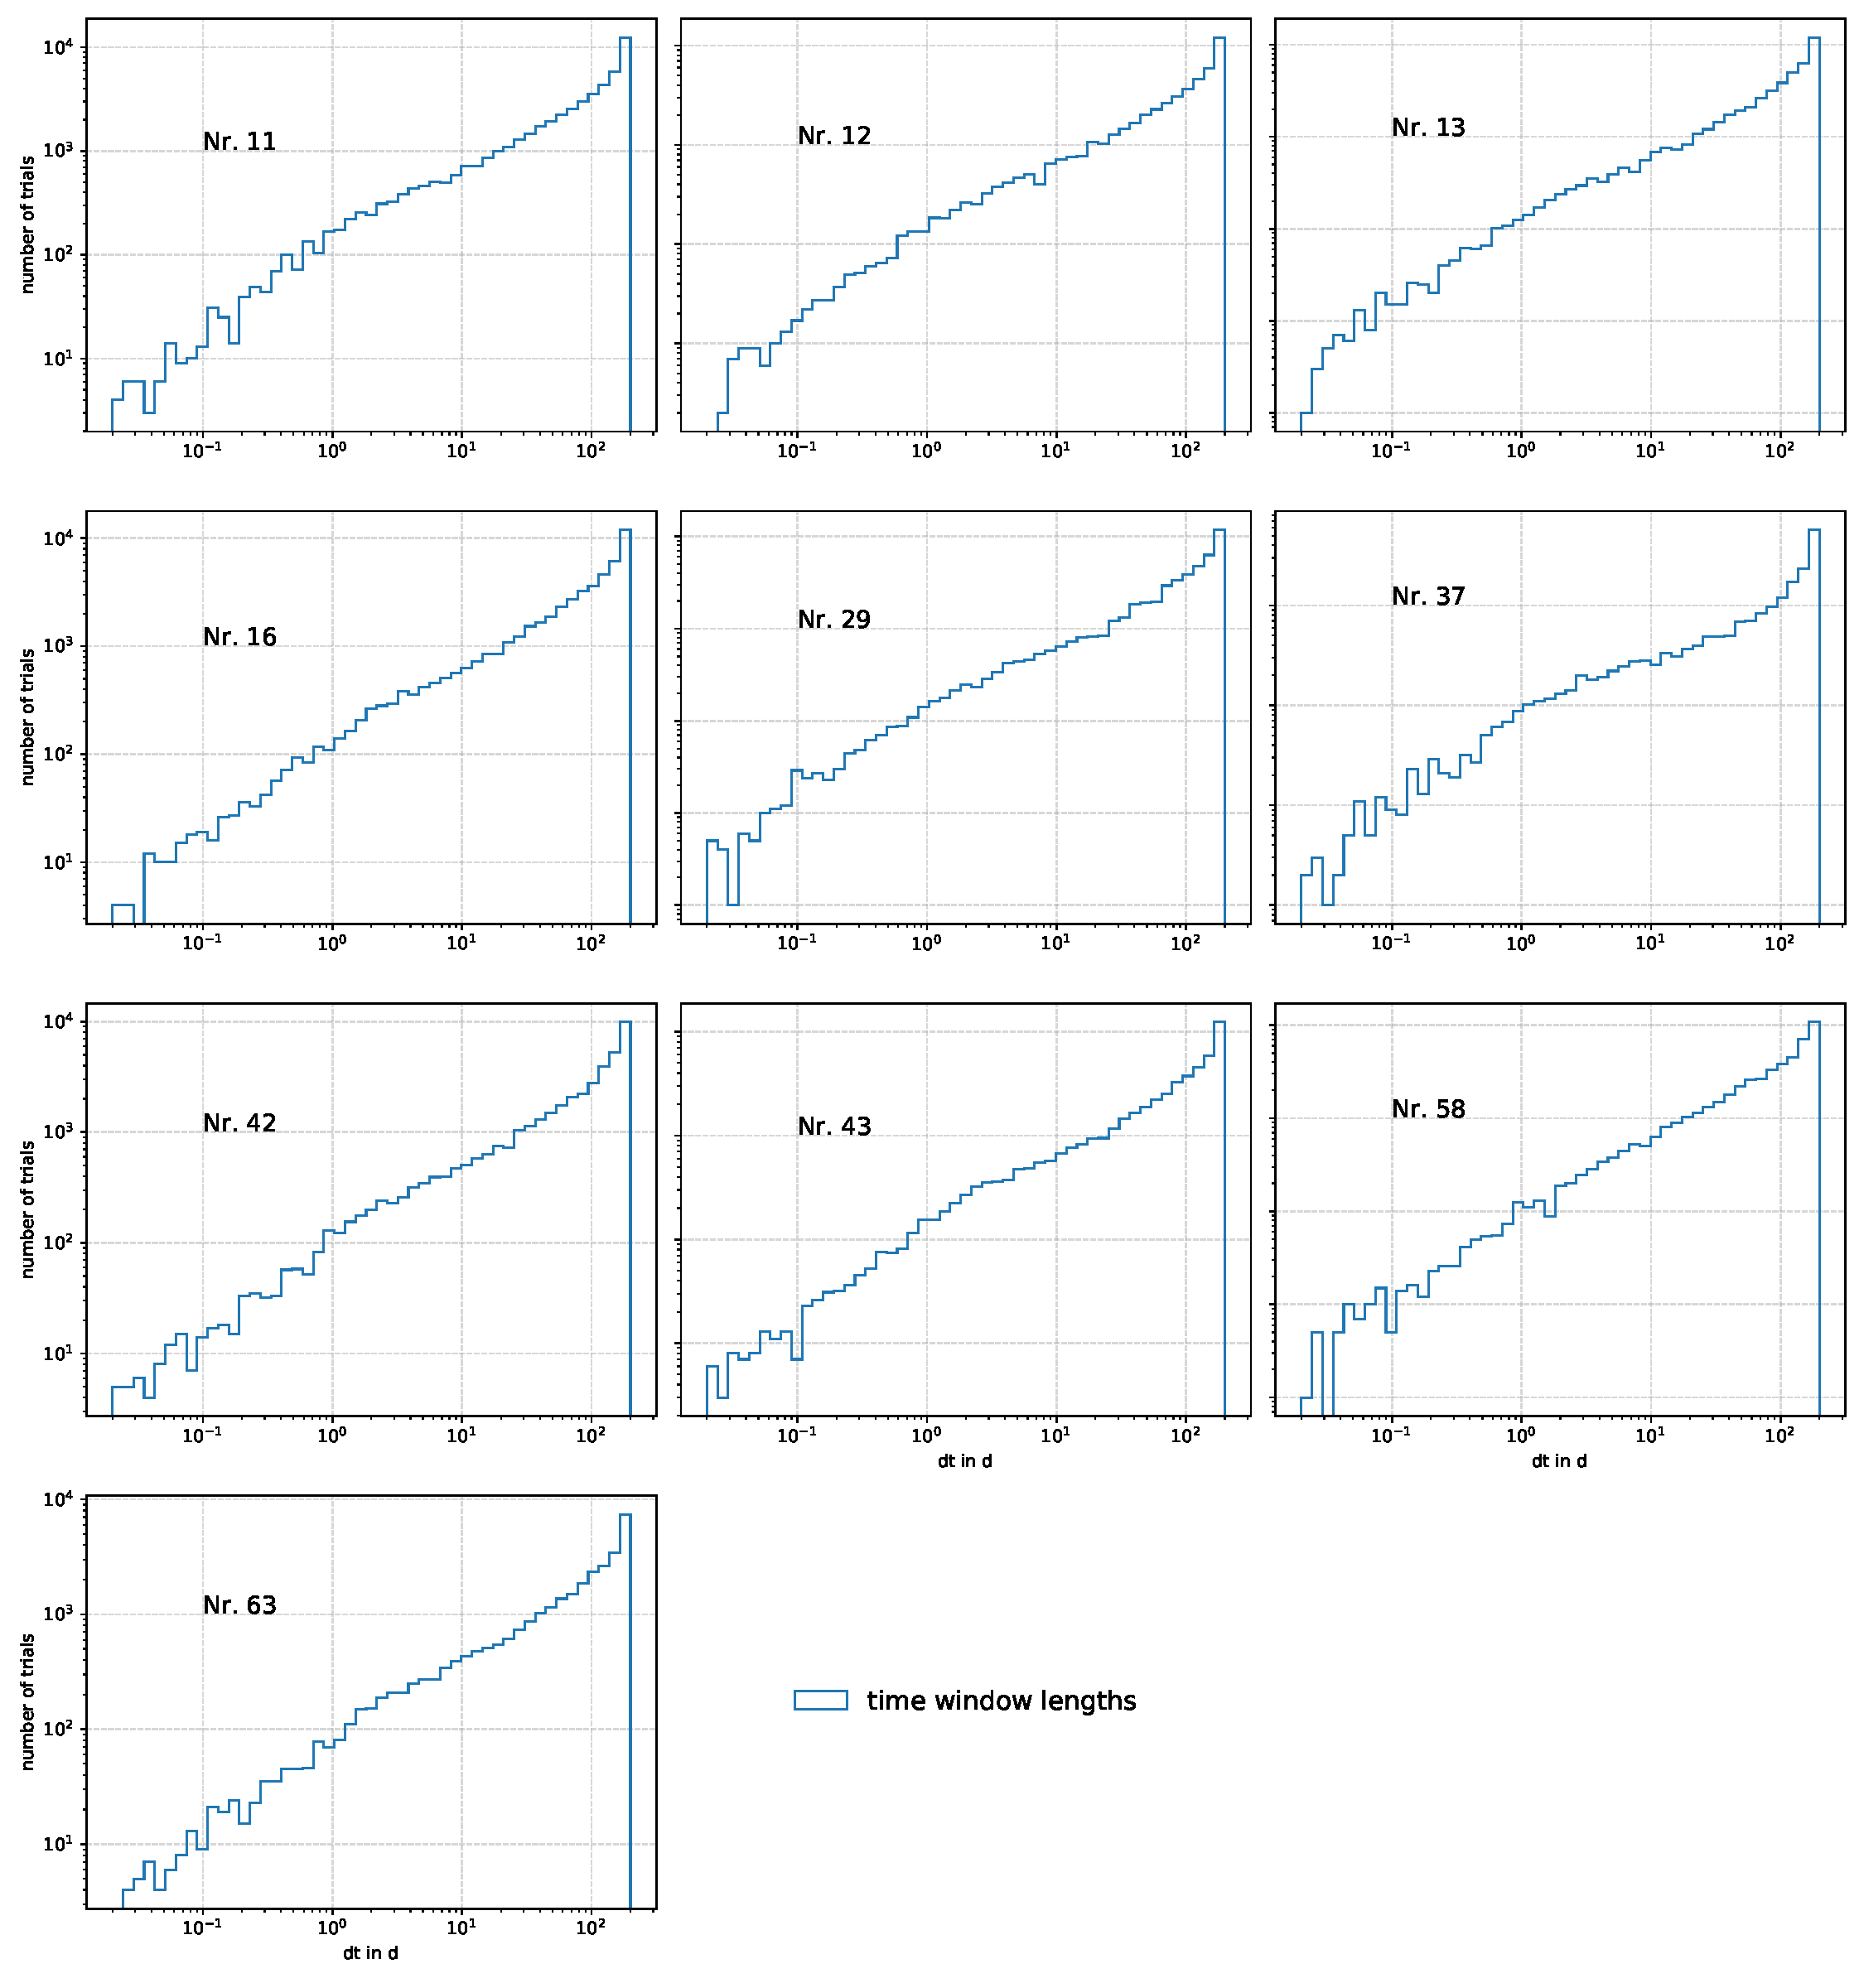
\includegraphics[width=\linewidth]{Plots/appendix/9_years_gfu_gold_time_dep_sens_dt.pdf}
    \caption{Histograms of the time window lengths $dt$ in days of all $\num{10}$ sources for the time-dependent analysis for the set of signal trials with the number of injected signal events closest to satisfying the condition to calculate the sensitivity.}
    \label{fig:sens_dt_all}
\end{figure}

\begin{figure}
    \centering
    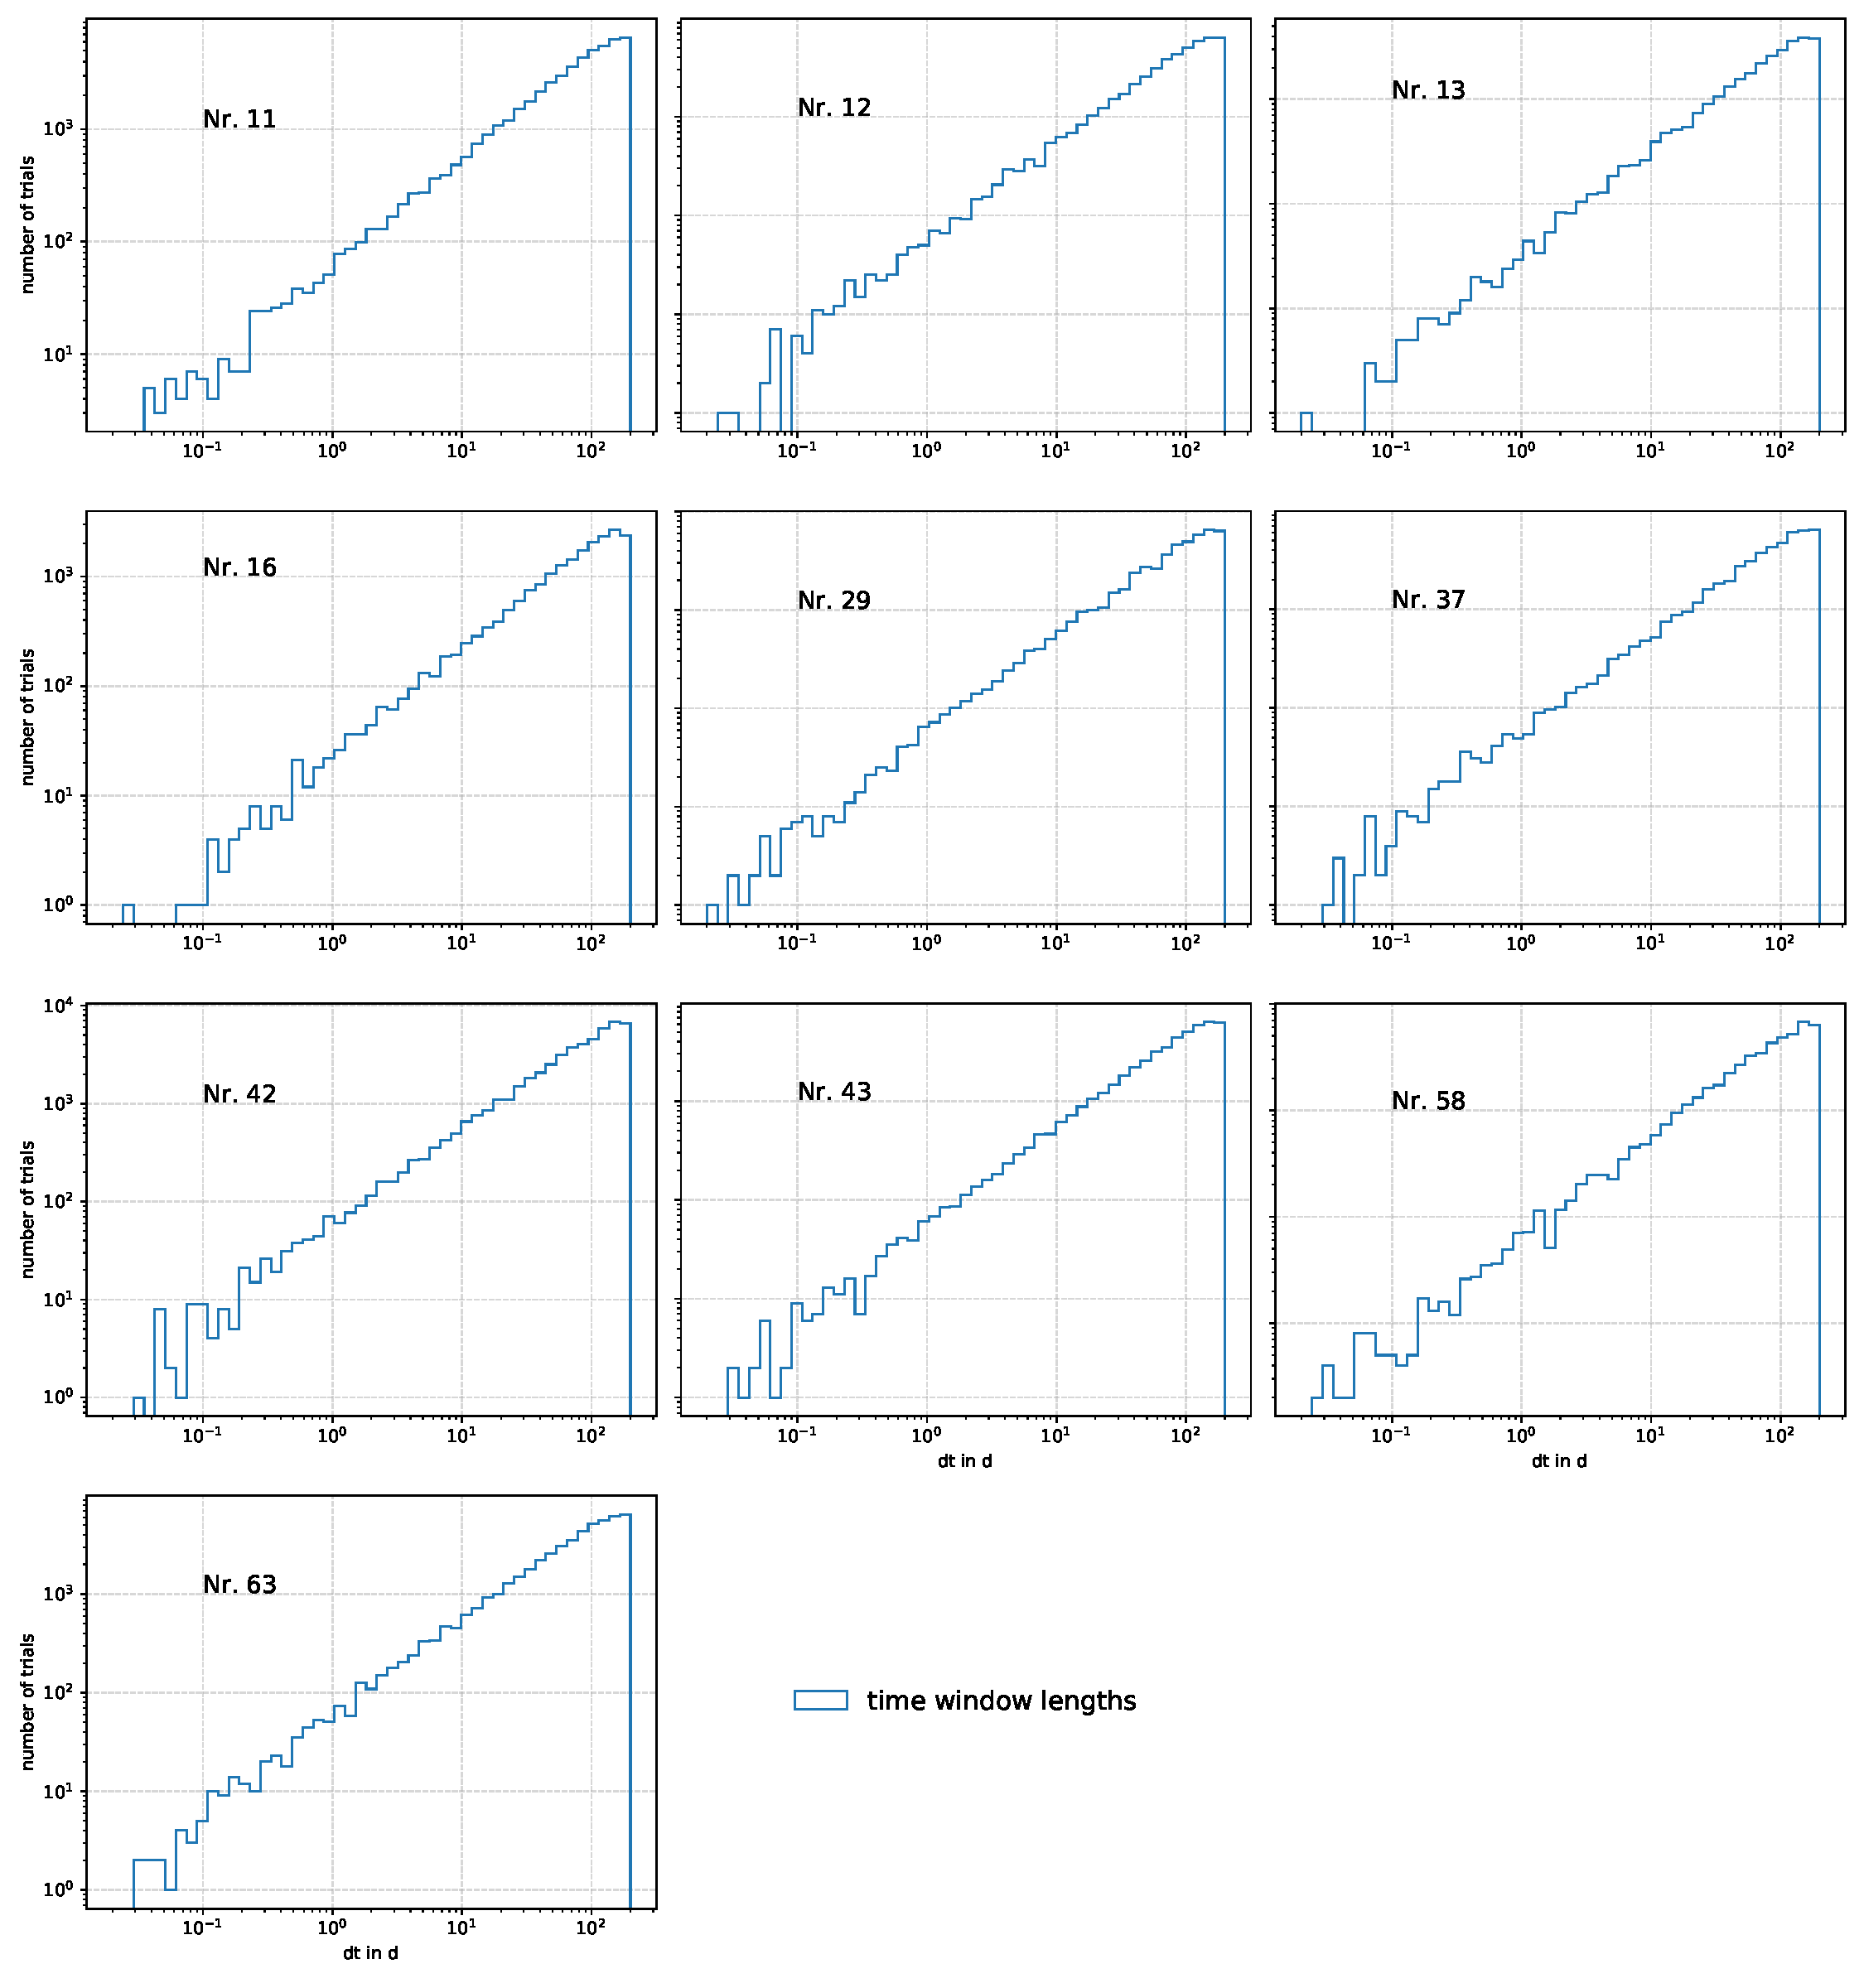
\includegraphics[width=\linewidth]{Plots/appendix/9_years_gfu_gold_time_dep_disc_dt.pdf}
    \caption{Histograms of the time window lengths $dt$ in days of all $\num{10}$ sources for the time-dependent analysis for the set of signal trials with the number of injected signal events closest to satisfying the condition to calculate the discovery potential.}
    \label{fig:disc_dt_all}
\end{figure}

\begin{figure}
    \centering
    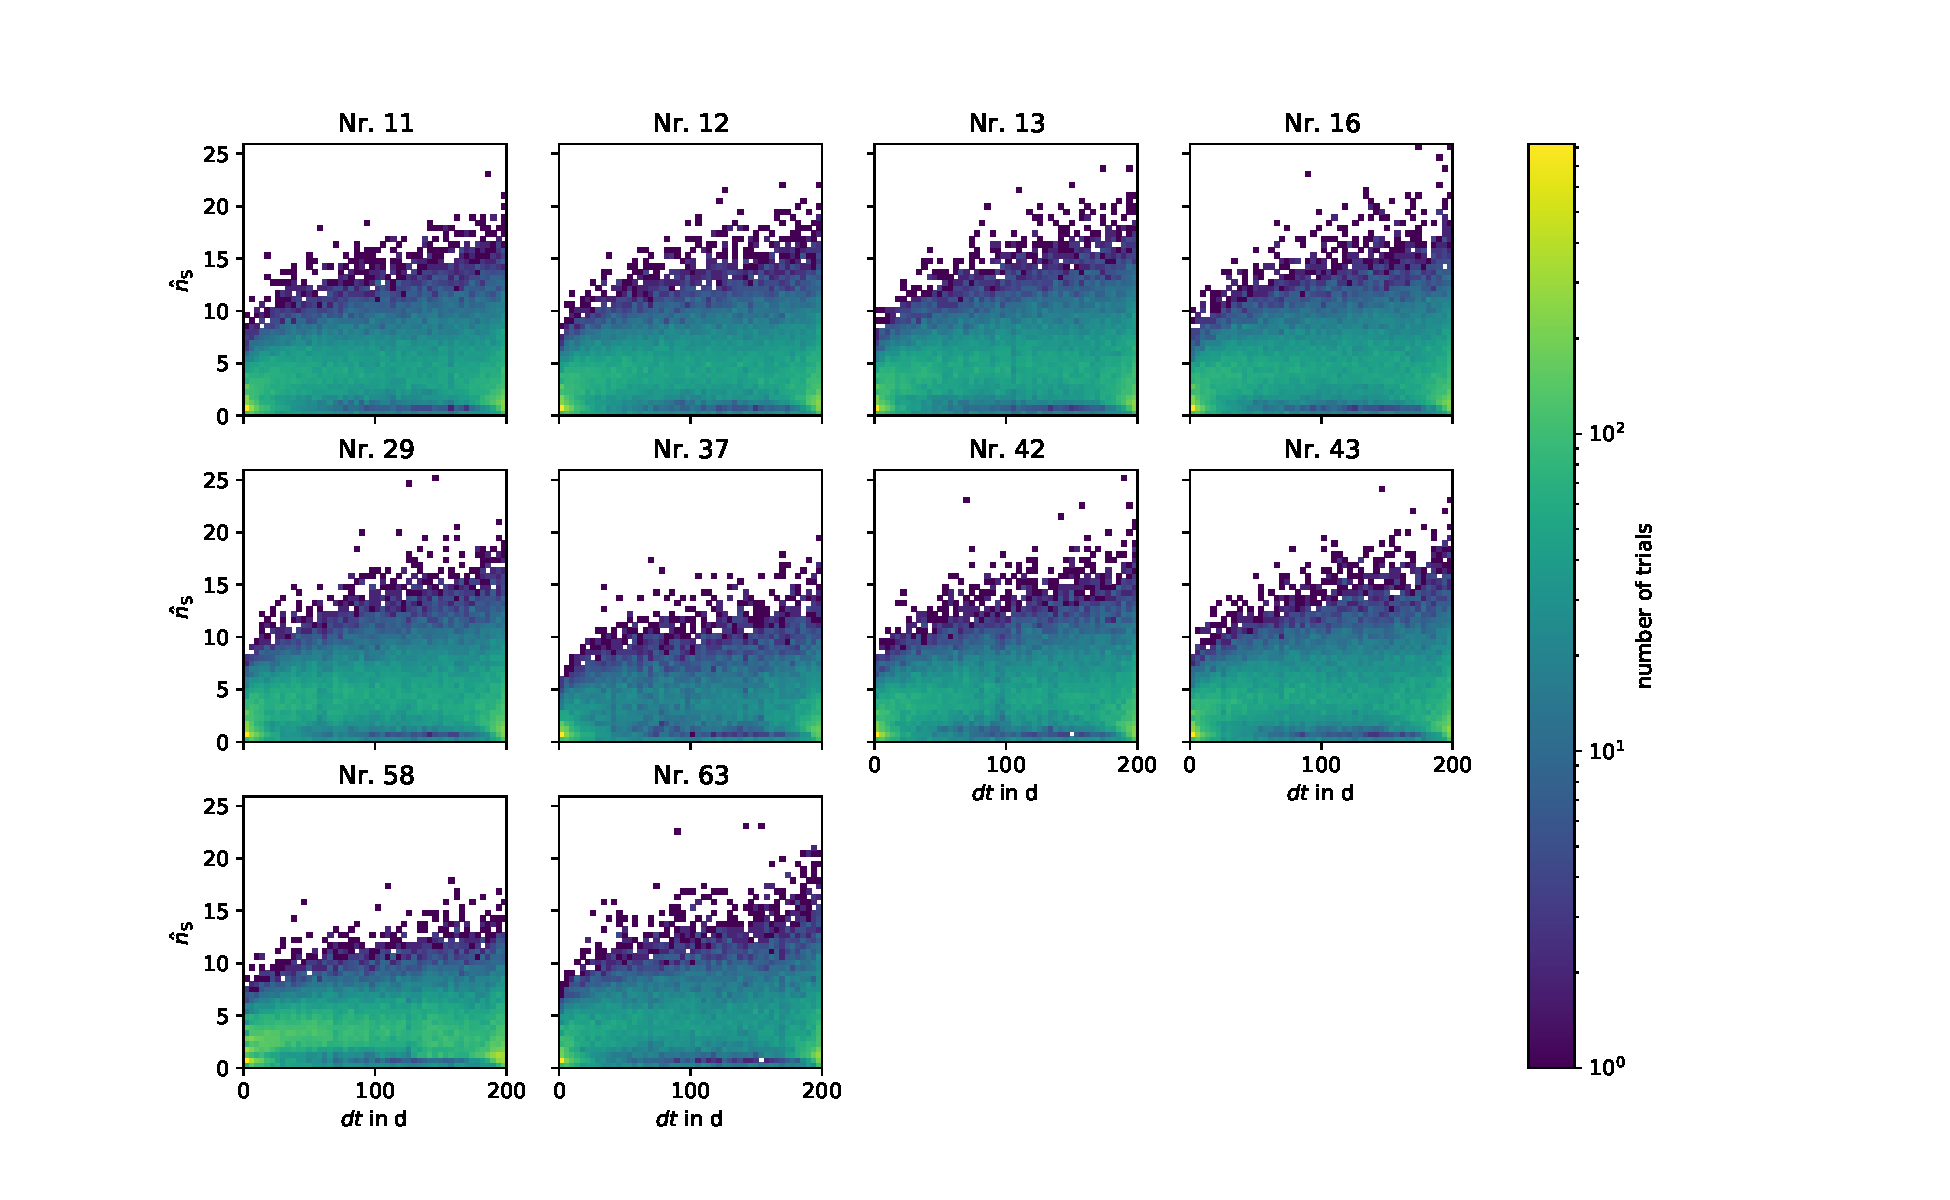
\includegraphics[width=\linewidth]{Plots/appendix/time_window_ns_sens_time_dep.pdf}
    \caption{Histograms of the time window lengths $dt$ in days in dependence of the fitted signal parameter $\hat{n}_\text{S}$ of all $\num{10}$ sources for the time-dependent analysis for the set of signal trials with the number of injected signal events closest to satisfying the condition to calculate the sensitivity.}
    \label{fig:sens_ns_dt_all}
\end{figure}

\begin{figure}
    \centering
    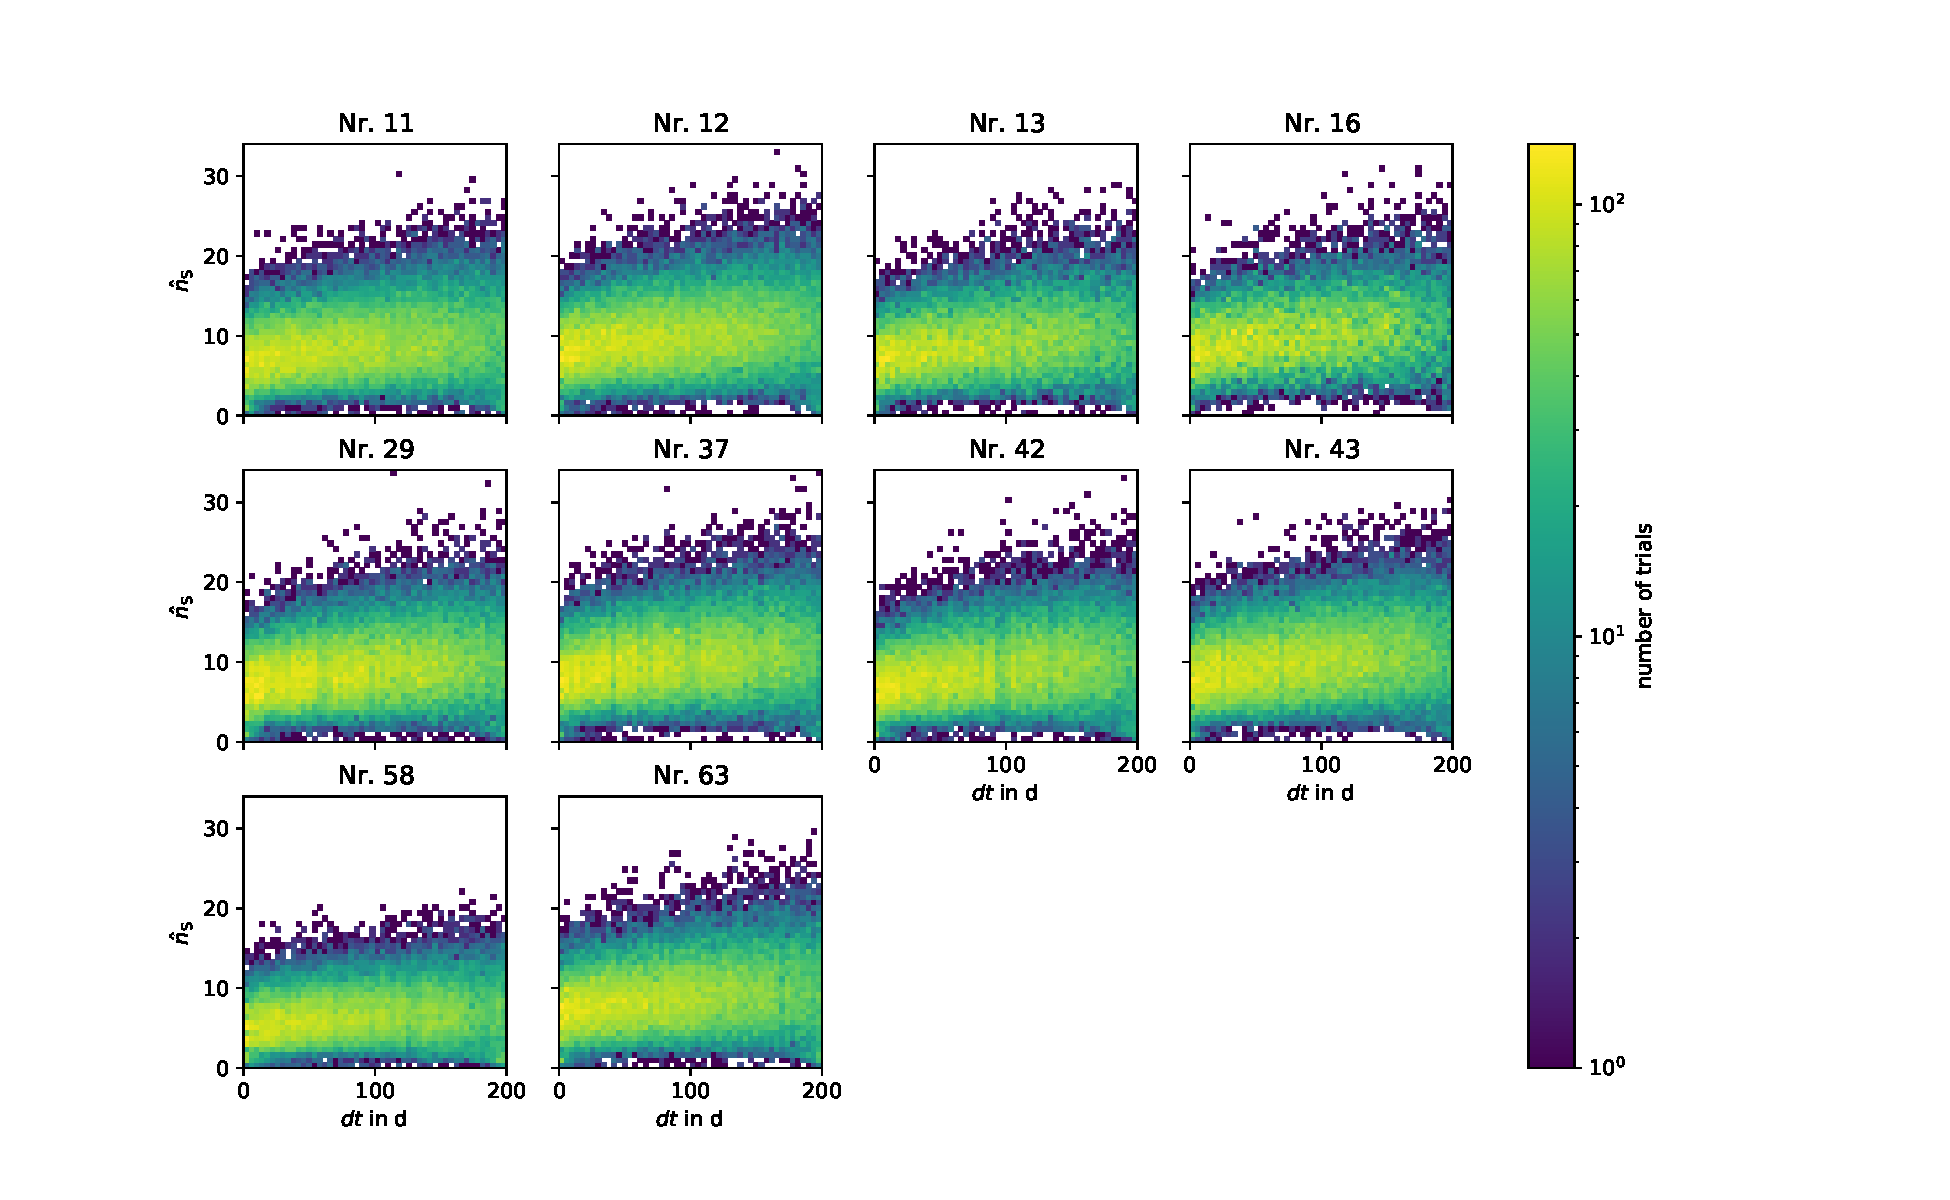
\includegraphics[width=\linewidth]{Plots/appendix/time_window_ns_disc_time_dep.pdf}
    \caption{Histograms of the time window lengths $dt$ in days in dependence of the fitted signal parameter $\hat{n}_\text{S}$ of all $\num{10}$ sources for the time-dependent analysis for the set of signal trials with the number of injected signal events closest to satisfying the condition to calculate the discovery potential.}
    \label{fig:disc_ns_dt_all}
\end{figure}
